\subsection{Trigonometric functions}

\ifnum \value{printWorkedSols}=1 

\pgfplotsset{
    myaxistrigfunctions/.style={
        width=0.8\textwidth,
        height=0.3\textwidth,
        xlabel={\small$\theta$ [rad]},
        grid=both,
        grid style={line width=.1pt, draw=gray!10},
        major grid style={line width=.2pt,draw=gray!50},
        axis lines=middle,
        enlargelimits={abs=0.25},
        axis line style={latex-latex},
        ticklabel style={font=\small,fill=white},
    },
}

\begin{figure}[h]
    \centering
    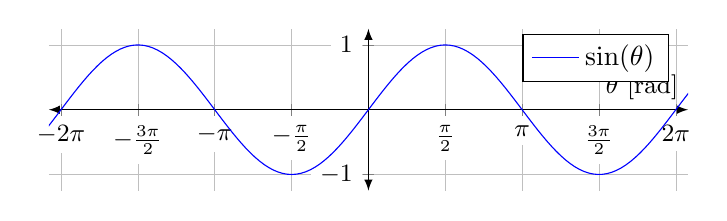
\begin{tikzpicture}
        \begin{axis}[
            myaxistrigfunctions,
            xmin=-2*pi, 
            xmax=2*pi,
            xtick={-2*pi, -3*pi/2, -pi, -pi/2, 0, pi/2, pi, 3*pi/2, 2*pi},
            xticklabels={$-2\pi$, $-\frac{3\pi}{2}$, $-\pi$, $-\frac{\pi}{2}$, $0$, $\frac{\pi}{2}$, $\pi$, $\frac{3\pi}{2}$, $2\pi$},
            domain=-3*pi:3*pi,
            samples=200,
            legend entries={$\sin(\theta)$},
            legend pos=north east,
        ]
            \addplot[blue] {sin(deg(x))};
        \end{axis}
    \end{tikzpicture}
    % \caption{Sine Function}
\end{figure}

% Cosine graph
\begin{figure}[h]
    \centering
    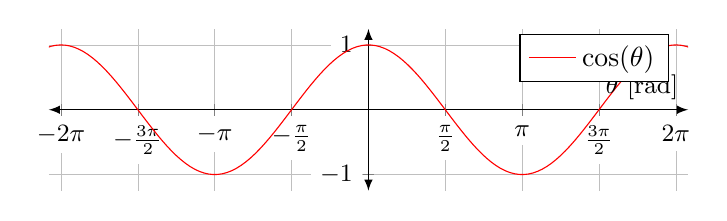
\begin{tikzpicture}
        \begin{axis}[
            myaxistrigfunctions,
            xmin=-2*pi, 
            xmax=2*pi,
            xtick={-2*pi, -3*pi/2, -pi, -pi/2, 0, pi/2, pi, 3*pi/2, 2*pi},
            xticklabels={$-2\pi$, $-\frac{3\pi}{2}$, $-\pi$, $-\frac{\pi}{2}$, $0$, $\frac{\pi}{2}$, $\pi$, $\frac{3\pi}{2}$, $2\pi$},
            domain=-3*pi:3*pi,
            samples=200,
            legend entries={$\cos(\theta)$},
            legend pos=north east,
        ]
            \addplot[red] {cos(deg(x))};
        \end{axis}
    \end{tikzpicture}
    % \caption{Cosine Function}
\end{figure}

% Tangent graph
\begin{figure}[h]
    \centering
    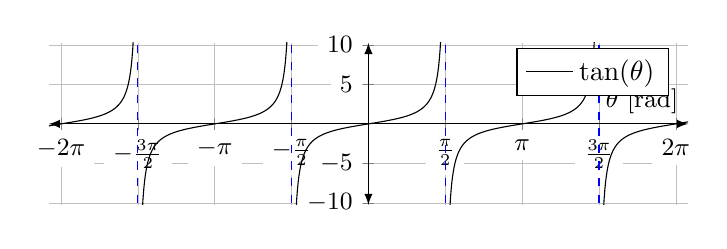
\begin{tikzpicture}
        \begin{axis}[
            myaxistrigfunctions,
            xmin=-2*pi, 
            xmax=2*pi,
			ymin=-10,
			ymax=10,
            xtick={-2*pi, -3*pi/2, -pi, -pi/2, 0, pi/2, pi, 3*pi/2, 2*pi},
            xticklabels={$-2\pi$, $-\frac{3\pi}{2}$, $-\pi$, $-\frac{\pi}{2}$, $0$, $\frac{\pi}{2}$, $\pi$, $\frac{3\pi}{2}$, $2\pi$},
            domain=-3*pi:3*pi,
            samples=100,
            legend entries={$\tan(\theta)$},
            legend pos=north east,
        ]
		\addplot[black, domain=-5*pi/2+0.01:-3*pi/2-0.01, samples=200] {tan(deg(x))};
		\addplot[black, domain=-3*pi/2+0.01:-pi/2-0.01, samples=200] {tan(deg(x))};
		\addplot[black, domain=-pi/2+0.01:pi/2-0.01, samples=200] {tan(deg(x))};
		\addplot[black, domain=pi/2+0.01:3*pi/2-0.01, samples=200] {tan(deg(x))};
		\addplot[black, domain=3*pi/2+0.01:5*pi/2-0.01, samples=200] {tan(deg(x))};
		% Asymptotes
		\draw[dashed, blue] (axis cs: -3*pi/2,-10) -- (axis cs: -3*pi/2,10);
		\draw[dashed, blue] (axis cs: -pi/2,-10) -- (axis cs: -pi/2,10);
		\draw[dashed, blue] (axis cs: pi/2,-10) -- (axis cs: pi/2,10);
		\draw[dashed, blue] (axis cs: 3*pi/2,-10) -- (axis cs: 3*pi/2,10);

        \end{axis}
    \end{tikzpicture}
    % \caption{Tangent Function}
\end{figure}

\fi
